\chapter{Planificación}\label{chap:Plan}
El presente capítulo mostrará la planificación que el proyecto se propone seguir, los recursos usados para su desarrollo así como una estimación del presupuesto que debería haber llevado consigo.

\section{Planificación temporal}
La sección actual se propone trazar un esquema temporal del trabajo a realizar. Al comienzo se hablará de la planificación que en un principio se pensaba seguir, para finalizar el capítulo con el calendario actualizado a la planificación que debió seguirse.

Previamente a todo ello, se describirá el modo en que hemos dividido el trabajo para poder ser divisible, mesurable y así asignable a un plan de tiempos.

\subsection{Paquetes de trabajo}
Dividiremos el trabajo total a realizar en distintos \textit{paquetes de trabajo} (para abreviar \texttt{P.i}, donde \texttt{i} es el número del paquete). A su vez, estos paquetes serán divididos en \textit{subtareas} (\texttt{S.i.j}, donde \texttt{j} es el número de la subtarea en el paquete) que concretan aún más el objeto del paquete. Pasamos a listar tanto paquetes como subtareas:

\subsubsection{P.1 Revisión bibliográfica}
Este paquete recoge las tareas relacionadas con el estudio previo de la materia que circunscribe todo el documento. Se trata de una tarea importa ya que sobre ella se cimentará todo el trabajo posterior. Un buen análisis del entorno nos posibilitará una mayor facilidad en la realización del proyecto.
\begin{itemize}
\item \textbf{S.1.1 Revisión bibliográfica sobre la educación y los videojuegos}. Pequeño estudio previo al trabajo para entender mejor la relación entre los videojuegos y su labor educativa.
\item \textbf{S.1.2 Revisión del estado actual de simuladores/emuladores de redes}. Investigación para encontrar cuáles son las aplicaciones encargadas de virtualizar redes más importantes y populares a día de hoy.
\item \textbf{S.1.3 Revisión del estado actual de los motores de juego}. Búsqueda de los motores para la fabricación de videojuegos. Tanto esta tarea como la anterior serán abordadas en el capítulo \ref{chap:ArtState}.
\item \textbf{S.1.4 Análisis de las tecnologías encontradas}. Tras las investigaciones previas, es necesario hacer un análisis de entre todas las tecnologías encontradas para quedarnos con aquellas que más nos convengan en función de las ventajas que presentan frente al resto. El análisis ha sido condensado en el capítulo \ref{chap:Analisis}.
\end{itemize}

\subsubsection{P.2 Diseño del proyecto}
El actual paquete tiene por misión crear un diseño previo a la implementación del propósito último del proyecto. Se trata de un esbozo de lo que en última instancia será desarrollado. Se estudia durante todo el capítulo \ref{chap:Design}.
\begin{itemize}
\item \textbf{S.2.1 Diseño del sistema de interconexión red-juego}. En este punto cabe investigar y proponer ideas acerca del modo en el que el juego es habilitado para interaccionar directamente con el simulador/emulador. Esto derivará en, como más tarde se verá, el diseño de una biblioteca en C\#.
\item \textbf{S.2.2 Diseño conceptual del juego}. Estructura que el juego debe contener así como ideas de niveles que puedan ser implementadas en él.
\end{itemize}

\subsubsection{P.3 Dominio de las herramientas}
Elegidas las tecnologías con las que llevar a cabo nuestro trabajo en S.1.4, queda aprender a usarlas. Es interesante en este punto buscar, para cada una de las tecnologías usadas, herramientas internas que puedan ayudarnos con nuestro fin.
\begin{itemize}
\item \textbf{S.3.1 Toma de contacto con el simulador de redes}. Es necesario conocerlo y comprenderlo, ya sea para poder usarlo junto al juego como para facilitar la realización de la herramienta que interconecta juego-simulador. Encontrar nodos compatibles con nuestro proyecto es igualmente importante.
\item \textbf{S.3.2 Lectura sobre las particularidades de C\#}. C\# es el lenguaje sobre el que se realizará la biblioteca que permitirá la interconexión entre juego y simulador. Se trata de un lenguaje de sintaxis similar a Java, con lo que no debe suponer una primera toma de contacto extremadamente compleja. Sin embargo, es necesario estudiarlo mínimamente para hacerse a él y sacarle todo el partido posible.
\item \textbf{S.3.3 Toma de contacto con el entorno de desarrollo del juego}. La inexperiencia con motores de juego requerirá pasar más tiempo en esta tarea.
\end{itemize}

\subsubsection{P.4 Implementación del diseño}
Tras el diseño, se procede a la implementación. Este proceso está extensamente redactado durante el capítulo \ref{chap:Integration}.
\begin{itemize}
\item \textbf{S.4.1 Creación de la biblioteca}. Hemos acordado que la herramienta que posibilita la interacción entre simulador y juego es una biblioteca llamada desde una API. Su desarrollo es lo que cubre esta tarea. 
\item \textbf{S.4.2 Creación del juego}. Desarrollo de un juego que satisfaga nuestras necesidades. Esto no solo incluye todo el desarrollo del juego en el motor que sea elegido (búsqueda de assets de arte, despliegue de objetos en las escenas, scripting) sino también la creación de las redes necesarias en el software de virtualización.
\end{itemize}

\subsubsection{P.5 Experimentación}
Tal y como podrá leerse en el capítulo \ref{chap:Pruebas}, este paquete contiene las tareas llevadas a cabo para analizar el trabajo llevado a cabo.
\begin{itemize}
\item \textbf{S.5.1 Creación de los escenarios de pruebas}. Dos son los escenarios sobre los que las pruebas se llevarán a cabo. Es necesario definirlos correctamente antes de que estas sean aplicadas.
\item \textbf{S.5.2 Ejecución de las pruebas}. Una serie de pruebas serán llevadas a cabo para comprobar la eficiencia del trabajo llevado a cabo.
\end{itemize}

\subsubsection{P.6 Redacción de la memoria}
Finalizado el trabajo, es momento de redactar todo el procedimiento seguido y los resultados obtenidos tras él. Como es natural, comprende todos las páginas que se encuentran en este documento.

\subsection{Planificación inicial}
Mostramos ahora, en la tabla \ref{tab:plan1}, la planificación que se pretendió seguir. A la izquierda de la tabla se muestran las tareas a realizar y, a su lado, la fecha de inicio, finalización y el número de días que hay entre ellas. El software con el que se ha llevado este planning no cuenta como días de trabajo los fines de semana así que no son contados en la columna de la derecha.

\begin{table}[H]
\centering
\begin{tabular}{cccc}
\rowcolor[HTML]{3531FF} 
{\color[HTML]{FFFFFF} \textbf{Paquetes de trabajo y subtareas}} & {\color[HTML]{FFFFFF} \textbf{Inicio}}   & {\color[HTML]{FFFFFF} \textbf{Final}}   & {\color[HTML]{FFFFFF} \textbf{Nº dias}} \\
\rowcolor[HTML]{FD6864} 
P.1                                                             & 20/02/18                                 & 14/03/18                                & 17                                      \\
\rowcolor[HTML]{FFCCC9} 
S.1.1                                                           & 20/02/18                                 & 23/02/18                                & 4                                       \\
\rowcolor[HTML]{FFCCC9} 
S.1.2                                                           & 20/02/18                                 & 2/03/18                                 & 9                                       \\
\rowcolor[HTML]{FFCCC9} 
S.1.3                                                           & 26/02/18                                 & 2/03/18                                 & 5                                       \\
\rowcolor[HTML]{FFCCC9} 
S.1.4                                                           & 3/03/18                                  & 14/03/18                                & 8                                       \\
\rowcolor[HTML]{FE996B} 
P.2                                                             & 17/03/18                                 & 27/04/18                                & 30                                      \\
\rowcolor[HTML]{FFCE93} 
S.2.1                                                           & 17/03/18                                 & 20/04/18                                & 25                                      \\
\rowcolor[HTML]{FFCE93} 
S.2.2                                                           & 22/03/18                                 & 27/04/18                                & 27                                      \\
\rowcolor[HTML]{FFFE65} 
P.3                                                             & 2/04/18                                  & 27/04/18                                & 20                                      \\
\rowcolor[HTML]{FFFC9E} 
{\color[HTML]{333333} S.3.1}                                    & {\color[HTML]{333333} 2/04/18}           & {\color[HTML]{333333} 13/04/18}         & {\color[HTML]{333333} 10}               \\
\rowcolor[HTML]{FFFC9E} 
{\color[HTML]{333333} S.3.2}                                    & {\color[HTML]{333333} 21/04/18}          & {\color[HTML]{333333} 25/04/18}         & {\color[HTML]{333333} 3}                \\
\rowcolor[HTML]{FFFC9E} 
{\color[HTML]{333333} S.3.3}                                    & {\color[HTML]{333333} 9/04/18}           & {\color[HTML]{333333} 27/04/18}         & {\color[HTML]{333333} 15}               \\
\rowcolor[HTML]{67FD9A} 
P.4                                                             & 1/05/18                                  & 23/07/18                                & 60                                      \\
\rowcolor[HTML]{9AFF99} 
S.4.1                                                           & 1/05/18                                  & 11/06/18                                & 30                                      \\
\rowcolor[HTML]{9AFF99} 
S.4.2                                                           & 11/06/18                                 & 23/07/18                                & 31                                      \\
\rowcolor[HTML]{38FFF8} 
P.5                                                             & 23/07/18                                 & 31/07/18                                & 7                                       \\
\rowcolor[HTML]{96FFFB} 
S.5.1                                                           & 23/07/18                                 & 26/07/18                                & 4                                       \\
\rowcolor[HTML]{96FFFB} 
S.5.2                                                           & 26/07/18                                 & 31/07/18                                & 4                                       \\
\rowcolor[HTML]{96FFFB} 
P.6                                                             & 1/08/18                                  & 31/08/18                                & 23                                      \\
\rowcolor[HTML]{000000} 
{\color[HTML]{FFFFFF} \textbf{Trabajo Fin de Grado}}            & {\color[HTML]{FFFFFF} \textbf{20/02/18}} & {\color[HTML]{FFFFFF} \textbf{4/09/18}} & {\color[HTML]{FFFFFF} \textbf{141}}    
\end{tabular}
\caption{Planificación inicial}
\label{tab:plan1}
\end{table}

Son a los últimos tres paquetes de trabajo a aquellos a los que más tiempo se ha dedicado. La documentación y toma de contacto de los primeros no requiere de tantas horas como el que lleva la implementación final (entre otras cosas, por los incovenientes que surgen del trabajo). Esto es más visible en la figura \ref{fig:gant1}, donde se muestra el diagrama de Gantt asociado.

\begin{figure}[H]
  \centering
  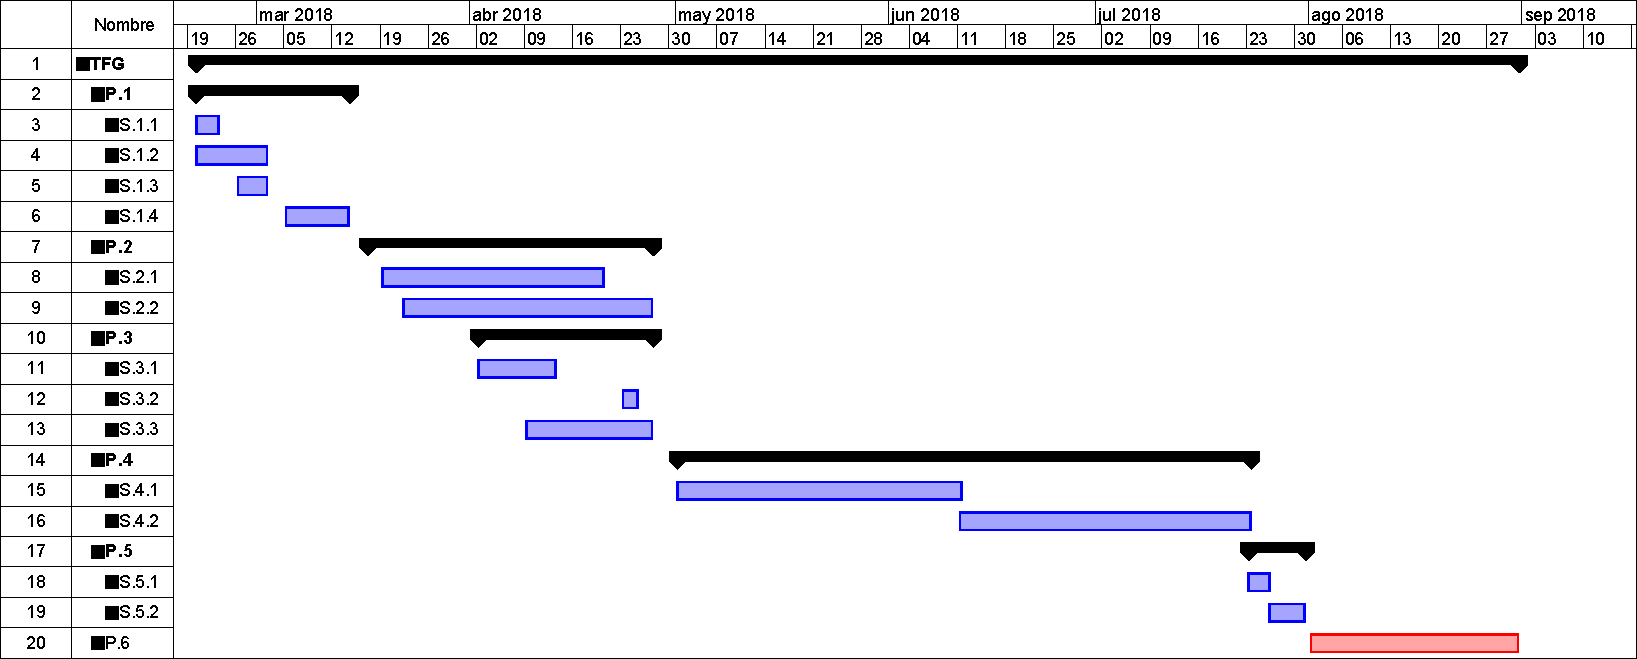
\includegraphics[scale=0.45]{imagenes/gant1}
  \caption{Diagrama de Gantt de la planificación inicial}
  \label{fig:gant1}
\end{figure}

\subsection{Planificación final}
Sin embargo, la anterior planificación no pudo seguirse con total exactitud. Circunstancias como los exámenes y las entregas presentes a final de cuatrimestre así como el comienzo en un nuevo empleo en junio, imposibilitaron llevarla a cabo. Así, aunque los paquetes de trabajo iniciales se mantienen más o menos estables, los referidos a la implementación, pruebas y redacción se alargaron y comprimieron hacia el final del calendario posible.

\begin{table}[H]
\centering
\begin{tabular}{cccc}
\rowcolor[HTML]{3531FF} 
{\color[HTML]{FFFFFF} \textbf{Paquetes de trabajo y subtareas}} & {\color[HTML]{FFFFFF} \textbf{Inicio}}   & {\color[HTML]{FFFFFF} \textbf{Final}}   & {\color[HTML]{FFFFFF} \textbf{Nº dias}} \\
\rowcolor[HTML]{FD6864} 
P.1                                                             & 20/02/18                                 & 14/03/18                                & 17                                      \\
\rowcolor[HTML]{FFCCC9} 
S.1.1                                                           & 20/02/18                                 & 23/02/18                                & 4                                       \\
\rowcolor[HTML]{FFCCC9} 
S.1.2                                                           & 20/02/18                                 & 2/03/18                                 & 9                                       \\
\rowcolor[HTML]{FFCCC9} 
S.1.3                                                           & 26/02/18                                 & 2/03/18                                 & 5                                       \\
\rowcolor[HTML]{FFCCC9} 
S.1.4                                                           & 3/03/18                                  & 14/03/18                                & 8                                       \\
\rowcolor[HTML]{FE996B} 
P.2                                                             & 17/03/18                                 & 27/04/18                                & 30                                      \\
\rowcolor[HTML]{FFCE93} 
S.2.1                                                           & 17/03/18                                 & 20/04/18                                & 25                                      \\
\rowcolor[HTML]{FFCE93} 
S.2.2                                                           & 22/03/18                                 & 27/04/18                                & 27                                      \\
\rowcolor[HTML]{FFFE65} 
P.3                                                             & 2/04/18                                  & 4/05/18                                 & 25                                      \\
\rowcolor[HTML]{FFFC9E} 
{\color[HTML]{333333} S.3.1}                                    & {\color[HTML]{333333} 2/04/18}           & {\color[HTML]{333333} 20/04/18}         & {\color[HTML]{333333} 15}               \\
\rowcolor[HTML]{FFFC9E} 
{\color[HTML]{333333} S.3.2}                                    & {\color[HTML]{333333} 21/04/18}          & {\color[HTML]{333333} 3/05/18}          & {\color[HTML]{333333} 9}                \\
\rowcolor[HTML]{FFFC9E} 
{\color[HTML]{333333} S.3.3}                                    & {\color[HTML]{333333} 9/04/18}           & {\color[HTML]{333333} 4/05/18}          & {\color[HTML]{333333} 20}               \\
\rowcolor[HTML]{67FD9A} 
P.4                                                             & 5/06/18                                  & 27/08/18                                & 60                                      \\
\rowcolor[HTML]{9AFF99} 
S.4.1                                                           & 5/06/18                                  & 24/08/18                                & 59                                      \\
\rowcolor[HTML]{9AFF99} 
S.4.2                                                           & 9/07/18                                  & 27/08/18                                & 36                                      \\
\rowcolor[HTML]{38FFF8} 
P.5                                                             & 28/08/18                                 & 31/08/18                                & 4                                       \\
\rowcolor[HTML]{96FFFB} 
S.5.1                                                           & 28/08/18                                 & 29/08/18                                & 2                                       \\
\rowcolor[HTML]{96FFFB} 
S.5.2                                                           & 30/08/18                                 & 31/08/18                                & 2                                       \\
\rowcolor[HTML]{96FFFB} 
P.6                                                             & 13/08/18                                 & 7/09/18                                 & 20                                      \\
\rowcolor[HTML]{000000} 
{\color[HTML]{FFFFFF} \textbf{Trabajo Fin de Grado}}            & {\color[HTML]{FFFFFF} \textbf{20/02/18}} & {\color[HTML]{FFFFFF} \textbf{7/09/18}} & {\color[HTML]{FFFFFF} \textbf{144}}    
\end{tabular}
\caption{Planificación final}
\label{tab:plan2}
\end{table}

\begin{figure}[H]
  \centering
  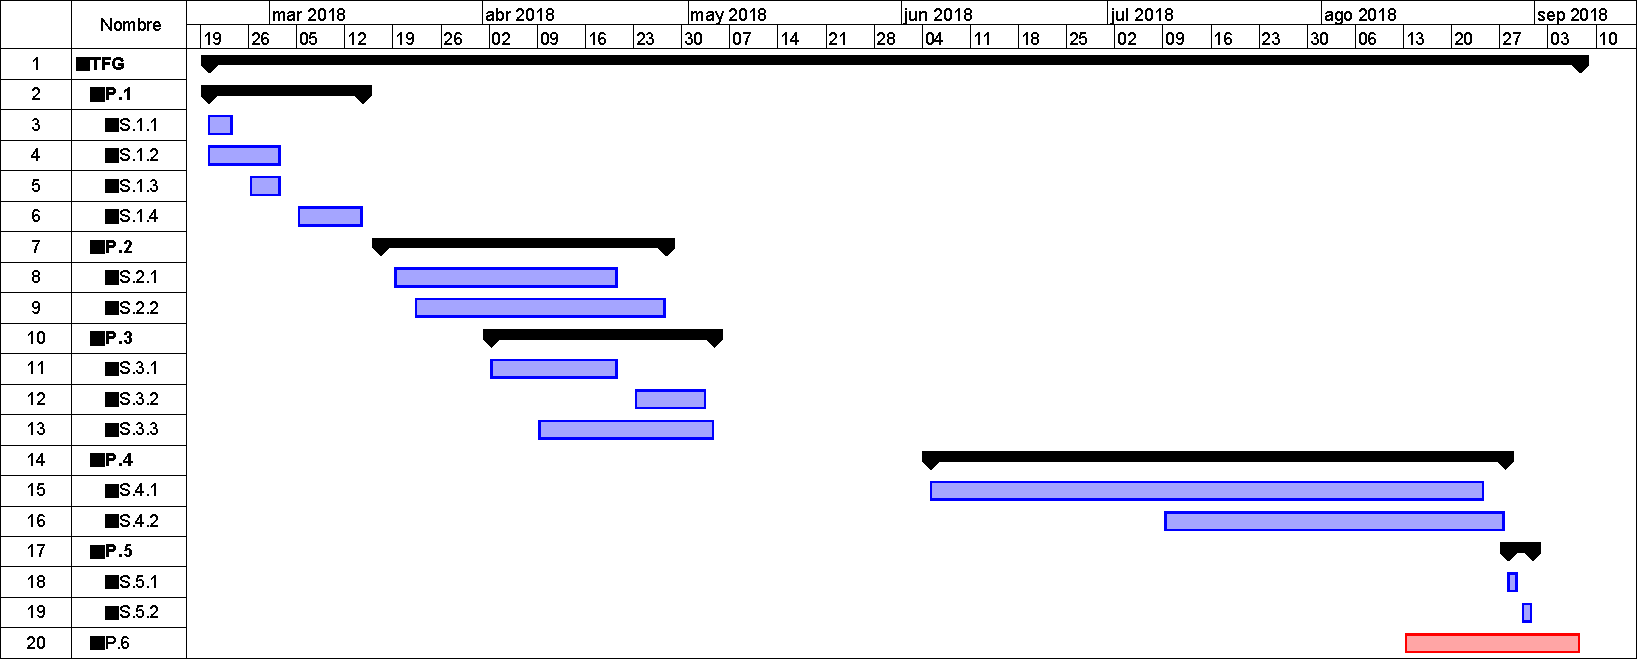
\includegraphics[scale=0.45]{imagenes/gant2}
  \caption{Diagrama de Gantt de la planificación final}
  \label{fig:gant2}
\end{figure}


\section{Recursos empleados}
Dividiremos los recursos utilizados para la realización del trabajo en tres: recursos humanos, recursos software y recursos hardware:

\subsection{Recursos humanos}
Aquí una lista de las personas que han participado en el proyecto y su papel en el mismo.
\begin{itemize}
\item Juan José Ramos Muñoz, profesor del departamento de Teoría de
la Señal, Telemática y Comunicaciones en la ETSIIT de la Universidad de Granada. Tutor del proyecto
\item Jonathan Prados Garzón, profesor del departamento de Teoría de
la Señal, Telemática y Comunicaciones en la ETSIIT de la Universidad de Granada.
Cotutor del proyecto.
\item Ángel Oreste Rodríguez Romero, alumno del grado de ingeniería de tecnologías de telecomunicación en la ETSIIT de la Universidad de Granada. Autor del proyecto.
\end{itemize}

\subsection{Recursos software}
Aplicaciones y demás material digital que ha sido necesario para desarrollar el trabajo:
\begin{itemize}
\item \href{https://www.microsoft.com/es-es/windows}{\textbf{Microsoft Windows 10 Home versión 1803}} como sistema operativo sobre el que se ha llevado todo el proyecto a cabo.
\item Se usará además \href{https://xubuntu.org/about/}{\textbf{Xubuntu 18.04}} instalado en una máquina virtual para llevar ciertas pruebas del capítulo \ref{chap:Pruebas} a cabo.
\item \href{https://www.mozilla.org/es-ES/firefox/}{\textbf{Mozilla Firefox Quantum}} como navegador web. 61.0.2 es la última versión empleada.
\item Para la realización de la memoria:
\begin{itemize}
\item El editor \href{http://www.xm1math.net/texmaker/}{\textbf{Texmaker 5.0.2}} junto a \href{https://miktex.org/about}{MiKTeX 2.9}, implementación de \LaTeX.
\item \href{https://es.libreoffice.org/descubre/draw/}{\textbf{LibreOffice Draw 6.1.0.3}} para el diseño de algunos esquemas.
\item \href{https://inkscape.org/es/}{\textbf{InkScape 0.92}} para la transformación de imágenes vectoriales en archivos de formato \textit{.pdf} y edición de las mismas.
\item Finalmente, la planificación ha requerido del uso del software \href{http://www.projectlibre.com/}{\textbf{ProjectLibre 1.7 Community Edition}}.
\end{itemize}
\item Como lector de archivos \textit{.pdf} ha sido elegido \href{https://www.foxitsoftware.com/pdf-reader/}{\textbf{Foxit Reader}}. Última versión: 9.2.0.
\item Para el desarrollo de código:
\begin{itemize}
\item El editor más utilizado durante el transcurso del trabajo ha sido \href{https://code.visualstudio.com/}{\textbf{Visual Studio Code}}. Ha pasado por varias versiones durante su uso. La más reciente es 1.26.
\item Para la compilación de código y el scripting en Unity el hermano mayor del anterior, \href{https://visualstudio.microsoft.com/es/}{\textbf{Microsoft Visual Studio Community}}, también ha pasado por varias versiones, pero la última de ellas ha sido la 15.8.0.
\item \href{https://notepad-plus-plus.org/}{\textbf{Notepad++}} ha sido utilizado para tomar notas y revisar código de forma rápida y ligera. La última versión usada es la 7.5.8.
\item \href{https://www.visual-paradigm.com/}{Visual Paradigm Enterprise 15.1} para dibujar los diagramas UML.
\end{itemize}
\item Para la virtualización de redes:
\begin{itemize}
\item \href{https://www.gns3.com/}{\textbf{GNS3 2.1.3 y finalmente 2.1.9}} como simulador de redes.
\item \href{https://www.virtualbox.org/}{\textbf{VirtualBox 5.2.16}} para la virtualización de ciertos dispositivos de la red y la instalación de un sistema Linux (Xubuntu) en el que integrar GNS3.
\end{itemize}
\item El motor para el desarrollo de videojuegos \href{https://unity3d.com/es}{\textbf{Unity}} versión personal. El último número de versión empleado ha sido el 2018.2.2f1.
\item Para el capítulo \ref{chap:Pruebas} serán útiles \href{https://docs.microsoft.com/en-us/sysinternals/downloads/rammap}{\textbf{RamMap 1.51}} y \href{https://docs.microsoft.com/en-us/sysinternals/downloads/process-explorer}{\textbf{Process Explorer 16.21}}.
\end{itemize}

\subsection{Recursos hardware}
Todo el proyecto ha sido construido a través del portátil Lenovo Z500. Cuenta con un procesador Intel i7 3232QM de ocho núcleos virtuales, 16GB de RAM DDR3 a 798MHz, un disco duro HDD de 1GB a 5400RPM y una tarjeta gráfica dedicada Nvidia 740M con 1GB VRAM. Los últimos meses también se ha hecho uso de un monitor \href{https://www.benq.es/product/monitor/gw2470h/}{BenQ GW2470H}, el cual ha facilitado enormemente todo el trabajo.

\section{Presupuesto}
Finalmente, haciendo una estimación de las horas trabajadas gracias a la planificación y mediante un análisis del inventario de los recursos empleados, podemos estimar un presupuesto asociado al trabajo.

Sin lugar a dudas, el pico económico se encuentra en la mano de obra humana. Hemos hecho una estimación del número de horas empleadas en el proyecto y, asignándole un precio a cada una de ellas, se ha hecho el cálculo que junto al resto del presupuesto puede verse en la tabla \ref{tab:presupuesto}.

Se buscó en todo momento que el software empleado fuera libre (ya sea por seguir la filosofía \textit{open source}, ya sea por disminuir gastos), de modo que el presupuesto total se reduce considerablemente.

\begin{table}[H]
\centering
\begin{tabular}{ccc}
\rowcolor[HTML]{3531FF} 
{\color[HTML]{FFFFFF} \textbf{Elemento}}                          & {\color[HTML]{FFFFFF} \textbf{Coste}}    & {\color[HTML]{FFFFFF} \textbf{Coste total}} \\
Trabajo alumno                                                    & 20\euro/hora                                 & 8640\euro                                       \\
\rowcolor[HTML]{EFEFEF} 
\begin{tabular}[c]{@{}c@{}}Trabajo tutor\\ y cotutor\end{tabular} & 40\euro/hora                                 & 800\euro                                        \\
\begin{tabular}[c]{@{}c@{}}PC con Windows\\ 10 Home\end{tabular}  & 750\euro                                     & 750\euro                                        \\
\rowcolor[HTML]{EFEFEF} 
Línea de internet                                                 & 15\euro/mes                                  & 120\euro                                        \\
Monitor                                                           & 130\euro                                     & 130\euro                                        \\
\rowcolor[HTML]{EFEFEF} 
Resto de software                                                 & 0\euro                                       & 0\euro                                          \\
\rowcolor[HTML]{000000} 
{\color[HTML]{FFFFFF} \textbf{Trabajo Fin de Grado}}              & {\color[HTML]{FFFFFF} -} & {\color[HTML]{FFFFFF} \textbf{10440\euro}}    
\end{tabular}
\caption{Presupuesto}
\label{tab:presupuesto}
\end{table}